\tikzset{every picture/.style={line width=0.75pt}} %set default line width to 0.75pt        

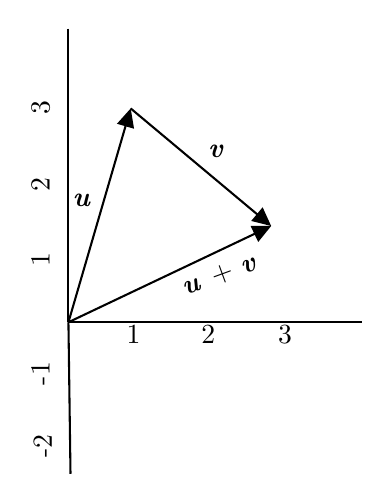
\begin{tikzpicture}[x=0.75pt,y=0.75pt,yscale=-1,xscale=1]
%uncomment if require: \path (0,218); %set diagram left start at 0, and has height of 218


%Shape: Boxed Line [id:dp4197928522176406] 
\draw    (296,5.29) -- (296,146.71) ;
%Shape: Boxed Line [id:dp1386254206809665] 
\draw    (437.42,146.71) -- (296,146.71) ;

%Straight Lines [id:da9069771914880562] 
\draw    (296,146.71) -- (325.16,46.59) ;
\draw [shift={(326,43.71)}, rotate = 466.24] [fill={rgb, 255:red, 0; green, 0; blue, 0 }  ][line width=0.08]  [draw opacity=0] (8.93,-4.29) -- (0,0) -- (8.93,4.29) -- cycle    ;
%Shape: Boxed Line [id:dp25011998260574986] 
\draw    (296,146.71) -- (297,219.71) ;
%Straight Lines [id:da6475776498837635] 
\draw    (326,43.71) -- (391.37,98.41) ;
\draw [shift={(393.67,100.34)}, rotate = 219.92000000000002] [fill={rgb, 255:red, 0; green, 0; blue, 0 }  ][line width=0.08]  [draw opacity=0] (8.93,-4.29) -- (0,0) -- (8.93,4.29) -- cycle    ;
%Straight Lines [id:da29394742031612564] 
\draw    (296,146.71) -- (390.96,101.62) ;
\draw [shift={(393.67,100.34)}, rotate = 514.6] [fill={rgb, 255:red, 0; green, 0; blue, 0 }  ][line width=0.08]  [draw opacity=0] (8.93,-4.29) -- (0,0) -- (8.93,4.29) -- cycle    ;


% Text Node
\draw (327.38,147) node [anchor=north] [inner sep=0.75pt]   [align=left] {1};
% Text Node
\draw (363.38,147) node [anchor=north] [inner sep=0.75pt]   [align=left] {2};
% Text Node
\draw (400.38,147) node [anchor=north] [inner sep=0.75pt]   [align=left] {3};
% Text Node
\draw (276.87,43.5) node [anchor=north] [inner sep=0.75pt]  [rotate=-270] [align=left] {3};
% Text Node
\draw (276.88,80.5) node [anchor=north] [inner sep=0.75pt]  [rotate=-270] [align=left] {2};
% Text Node
\draw (276.88,116.5) node [anchor=north] [inner sep=0.75pt]  [rotate=-270] [align=left] {1};
% Text Node
\draw (309,92.21) node [anchor=south east] [inner sep=0.75pt]   [align=left] {\textbf{\textit{u}}};
% Text Node
\draw (276.87,171.5) node [anchor=north] [inner sep=0.75pt]  [rotate=-270] [align=left] {\mbox{-}1};
% Text Node
\draw (277.88,206.5) node [anchor=north] [inner sep=0.75pt]  [rotate=-270] [align=left] {\mbox{-}2};
% Text Node
\draw (361.83,69.03) node [anchor=south west] [inner sep=0.75pt]   [align=left] {\textbf{\textit{v}}};
% Text Node
\draw (347.74,125.66) node [anchor=north west][inner sep=0.75pt]  [rotate=-339.94] [align=left] {\textbf{\textit{u }}+ \textbf{\textit{v}}};


\end{tikzpicture}
